\documentclass{article}
\usepackage{graphicx}
\usepackage{amsmath,amsthm,amssymb}
\usepackage[font=small,labelfont=bf]{caption}
\usepackage{tikz}
\usepackage{pgfplots}
\pgfplotsset{compat=1.18}
\usetikzlibrary{calc, angles, quotes, shapes.geometric, decorations.pathreplacing}
\usepackage{tkz-euclide}
\usepackage[inline]{asymptote}
\usepackage{float}
\usepackage[margin=1in]{geometry}
\usepackage{gensymb}
\usepackage[normalem]{ulem}
\usepackage{hyperref}
\hypersetup{
    colorlinks=true,
    linkcolor=blue,
    filecolor=magenta,      
    urlcolor=cyan,
    pdftitle={Overleaf Example},
    pdfpagemode=FullScreen,
    }
\usepackage{fancyhdr}
\pagestyle{fancy}
\fancyhead[R]{Enoch Yu}
\pagenumbering{gobble}
\usepackage{enumitem}
\newtheorem{theorem}{Theorem}[section]
\newtheorem{lemma}[theorem]{Lemma}
\newtheorem*{lemma*}{Lemma}
\newtheorem{sublemma}{Lemma}[section]
\newtheorem{proposition}{Proposition}
\newtheorem{corollary}{Corollary}[theorem]
\newtheorem{example}{Example}[section]
\newtheorem*{example*}{Example}
\newenvironment{solution}{\begin{trivlist}\item[]{\bf Solution}}{\qed \end{trivlist}}
\newcommand{\verteq}{\rotatebox{90}{$\;\;=\;\;$}}
\newcommand*\circled[1]{\tikz[baseline=(char.base)]{
            \node[shape=circle,draw,inner sep=1pt] (char) {#1};}}
\newcommand{\triangled}[1]{\tikz[baseline=(char.base)]{
            \node[shape=regular polygon, regular polygon sides=3, draw, inner sep=0.2pt] (char) {#1};}}

\title{Problem Set 15}
\author{Enoch Yu}
\date{June 2025}

\begin{document}

\section*{Problem}
$A$, $B$, $C$, and $D$ stand in a circle. Simultaneously, each player selects another player at random and points at that person, who must then sit down. What is the probability that $A$ is the only person who remains standing?
\begin{solution}
\\\\
\textbf{Key Word} Counting Strategy
\\\\
\textbf{Solution I} \\
\begin{align*}
\text{total cases of only $A$ standing}&=\text{total cases of $A$ standing}-\text{total cases of $A$ and $(B,C,\text{ or }D)$ standing} \\
&=\frac{3}{3}\cdot\frac{2}{3}\cdot\frac{2}{3}\cdot\frac{2}{3}-\frac{2}{3}\cdot\frac{2}{3}\cdot\frac{1}{3}\cdot\frac{1}{3}\cdot{}_3C_2 \\
&=\frac{8}{27}-\frac{4}{27} \\
&=\boxed{\frac{4}{27}}
\end{align*}
\\\\
\textbf{Solution II} \\
\[
\begin{array}{cccc}
    A & B & C & D \\
    \hline
    B & C & D & B \\
      &   &   & C \\
      & D &   &   \\
    C \\
    D \\
\end{array}
\]
\[
\therefore\ \text{total cases of only $A$ standing}=\frac{3\cdot2\cdot1\cdot2}{3^4}=\boxed{\frac{4}{27}}
\]
\end{solution}

\newpage
\section*{Problem}
$R$ is blindfolded and standing 1 step away from an ice cream stand. Every second, he has a $\frac{1}{4}$ probability of walking 1 step towards the ice cream stand, and a $\frac{3}{4}$ probability of walking 1 step away from the ice cream stand. When he is 0 steps away from the ice cream stand, he wins. What is the probability that $R$ eventually wins?
\begin{solution}
\\\\
\textbf{Key Word} Recursion
\\\\
First and foremost, variables for recursion formula could be set.
\begin{align*}
    S_1&=\text{Probability to win from 1} \\
    S_2&=\text{Probability to win from 2} \\
    &\ \ \ \ \ \ \ \ \ \ \ \ \ \ \ \ \ \ \ \ \ \ \vdots
\end{align*}
Using the defined variables, recursion equations could be set.
\begin{align*}
    S_1&=\frac{1}{4}+\frac{3}{4}S_2 \\
    S_2&=\frac{1}{4}S_1+\frac{3}{4}S_3 \\
    S_3&=\frac{1}{4}S_2+\frac{3}{4}S_4 \\
    &\ \ \ \ \ \ \ \ \ \ \ \ \vdots \\
    S_n&=\frac{1}{4}S_{n-1}+\frac{3}{4}S_{n+1} \\
\end{align*}
Notice that $S_1$ is the value that need to be computed since $R$ is located at 1.
\[
S_1+S_2+\dots+S_n=\frac{1}{4}+\frac{1}{4}(S_1+S_2+\dots+S_{n-1})+\frac{3}{4}(S_2+\dots+S_{n+1})
\]
For simplicity, let $A=S_1+S_2+\dots+S_n$.
\begin{align*}
A&=\frac{1}{4}+\frac{1}{4}(A-S_n)+\frac{3}{4}(A-S_1+S_{n+1}) \\
0&=1-S_n-3S_1+3S_{n+1}
\\\\
&\text{However, notice that }\lim_{n\rightarrow\infty}S_n=0.
\\\\
\therefore\ 0&=1-3S_1\\
S_1&=\boxed{\frac{1}{3}}
\end{align*}
\end{solution}

\newpage
\section*{Problem}
Enoch randomly hops between 5 leaves, on each turn hopping to one of the other 4 leaves with equal probability. After 5 hops, what is the probability that Enoch has returned to the leaf where he started?
\begin{solution}
\\\\
\textbf{Key Word} Recursion
\\\\
First and foremost, variables must be set in order to use recursion.
\begin{align*}
    h_x&=\text{Probability to be on the leaf where he started after $x$ hops} \\
    h_{x-1}&=\frac{1}{4}(1-h_{x-1})
\end{align*}
Using the formula above, substitution may lead to the correct answer.
\begin{align*}
    h_5&=\frac{1}{4}(1-h_4)=\boxed{\frac{51}{256}} \\
    h_4&=\frac{1}{4}(1-h_3)=\textcolor{red}{\frac{13}{64}} \\
    h_3&=\frac{1}{4}(1-h_2)=\textcolor{red}{\frac{3}{16}} \\
    h_2&=\frac{1}{4}(1-h_1)=\textcolor{red}{\frac{1}{4}} \\
    h_1&=0 \\
\end{align*}
\end{solution}

\newpage
\section*{Problem}
Let $ABCD$ be a unit square and let $X,Y,Z$ be points on sides $AB,BC,CD$, respectively, such that $AX=BY=CZ$. If the area of triangle $XYZ$ is $\frac{1}{3}$, what is the maximum value of the ratio $\frac{XB}{AX}$?
\begin{solution}
\\\\
\textbf{Key Word} Area Formula
\begin{center}
    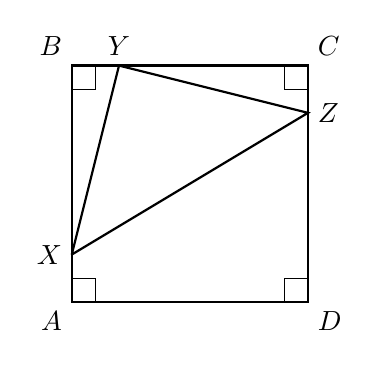
\begin{tikzpicture}[scale=3]
        \coordinate (A) at (0,0);
        \coordinate (B) at (0,1);
        \coordinate (C) at (1,1);
        \coordinate (D) at (1,0);
        
        \draw[thick] (A) -- (B) -- (C) -- (D) -- cycle;
        
        \node[below left] at (0,0) {$A$};
        \node[above left] at (0,1) {$B$};
        \node[above right] at (1,1) {$C$};
        \node[below right] at (1,0) {$D$};
        
        \coordinate (X) at (0,0.2);
        \coordinate (Y) at (0.2,1);
        \coordinate (Z) at (1,0.8);
        
        \draw[thick] (X) -- (Y) -- (Z) -- (X);
        
        \node[left] at (X) {$X$};
        \node[above] at (Y) {$Y$};
        \node[right] at (Z) {$Z$};
        
        \tkzMarkRightAngle[size=.1](A,B,C);
        \tkzMarkRightAngle[size=.1](B,C,D);
        \tkzMarkRightAngle[size=.1](C,D,A);
        \tkzMarkRightAngle[size=.1](D,A,B);
    \end{tikzpicture}
\end{center}
Let $AX=BY=CZ=a$.
\begin{align*}
    1-2\cdot\frac{a(1-a)}{2}-\frac{((1-a)+a)\cdot1}{2}&=\frac{1}{3} \\
    1-a(1-a)-\frac{1}{2}&=\frac{1}{3} \\
    a&=\frac{3\pm\sqrt3}{6}
    \\\\
    \text{The maximum value of }&\frac{1}{a}-1\text{ must be computed} \\
    \therefore\ \max\left(\frac{1}{a}-1\right)=\boxed{2+\sqrt{3}}
\end{align*}
\end{solution}

\end{document}
